\documentclass[12pt,letterpaper]{article}

%-----------------------------
%      PACKAGES & SETUP
%-----------------------------
\usepackage[margin=1in]{geometry}
\usepackage{amsmath,amssymb,amsfonts,bm}
\usepackage{graphicx}
\usepackage{booktabs}
\usepackage{enumitem}
\usepackage{float}
\usepackage{hyperref}
\usepackage{fancyhdr}
\usepackage{cite}
\usepackage{siunitx}
\usepackage{subcaption}
\usepackage{times}
\usepackage{xspace}
\usepackage{listings}
\usepackage{xcolor}

\usepackage[dvipsnames,svgnames,x11names]{xcolor} % full colour set + blends
\definecolor{linkblue}{HTML}{1A4B9B}   
\definecolor{citepink}{HTML}{AA0066}
\definecolor{urlteal}{HTML}{006D6D}

\hypersetup{
  colorlinks = true,
  linkcolor  = linkblue,     
  citecolor  = citepink,     
  urlcolor   = urlteal       
}

\usepackage{verbatim}

\setlength{\headheight}{14.5pt}
\pagestyle{fancy}
\fancyhf{}
\rhead{\thepage}
\lhead{CSE\,291 (SP\,2025) Miniproject}

\setlength{\parskip}{6pt}
\setlength{\parindent}{18pt}

% New commands and macros
\newcommand{\R}{\mathbb{R}}
\newcommand{\q}{\bm{q}}
\newcommand{\qd}{\dot{\bm{q}}}
\newcommand{\qdd}{\ddot{\bm{q}}}
\newcommand{\x}{\bm{x}}
\newcommand{\xd}{\dot{\bm{x}}}
\newcommand{\xdd}{\ddot{\bm{x}}}
\newcommand{\Lag}{\mathcal{L}}
\newcommand{\Mass}{\mathbf{M}}
\newcommand{\Damp}{\mathbf{C}}
\newcommand{\stiff}{\mathbf{K}}
\newcommand{\bfn}{\bm{n}}
\newcommand{\act}{\mathrm{act}}
\newcommand{\pent}{U_{\mathrm{contact}}}
\DeclareMathOperator{\diag}{diag}

\fancypagestyle{ack_footer}{
    \fancyhf{}
    \renewcommand{\headrulewidth}{0pt}
    \renewcommand{\footrulewidth}{0pt}
    \cfoot{
      \scriptsize
      \begin{minipage}[t]{0.95\textwidth}
      \textbf{Acknowledgments:} OpenAI's ChatGPT (model gpt-4o) was utilized to assist in adding comments and docstrings to Python functions, explain code implemented by me, ensure its correctness and alignment with equations of motion, and help debug code errors. The outputs were modified with major changes. I actively reviewed, tested, and adjusted the generated code and explanations to reflect my own understanding.
      \end{minipage}
    }
}

%% Additional colors and listings setup
\definecolor{lightgray}{gray}{0.95}
\definecolor{darkblue}{rgb}{0.0,0.0,0.5}

\lstset{
    backgroundcolor=\color{lightgray},
    basicstyle=\small\ttfamily,
    keywordstyle=\color{blue}\bfseries,
    commentstyle=\itshape\color{green!40!black},
    stringstyle=\color{red},
    columns=fullflexible,
    breaklines=true,
    frame=single,
    numbers=left,
    numbersep=5pt,
    showstringspaces=false,
    tabsize=4,
    captionpos=b,
    morekeywords={vector,rate,canvas,sphere,cylinder,distant_light,local_light,box,make_trail,trail_radius,trail_color,opacity}
}

\begin{document}

%===========================================================
%                     TITLE
%===========================================================
\begin{center}
    {\Large \textbf{Least-Action-Based Modeling and Rolling Locomotion \\ 
    of a Six-Strut Tensegrity Robot}}\\[10pt]
    \textbf{Param Somane}\\
    \emph{CSE 291 (Spring 2025) Midterm Miniproject}
\end{center}

\vspace{1em}

\begin{abstract}
\noindent
We present a comprehensive derivation and implementation of a six-strut \emph{tensegrity} robot capable of rolling locomotion. The robot's equations of motion are rigorously obtained via the Principle of Least Action, augmented with simple inequality constraints to model ground contact. We illustrate, step by step, how the system's node-based potential energy (including rods, cables, and a penalty-based contact formulation) fits within the Lagrangian framework, and how the final ODE set emerges from the stationary action condition. A time-integration scheme (an explicit fourth-order Runge--Kutta solver) is employed to simulate the dynamics in real time, and friction is incorporated as a separate (non-conservative) force. We further demonstrate how rolling gaits can be synthesized via a genetic algorithm optimizing each strut's actuation profile. Notably, while our primary exposition focuses on \emph{strut} (rod) telescoping, the \emph{code} currently actuates a subset of cables. We explain how this difference can be reconciled. This document meets the project requirement of describing the system, deriving its equations of motion under contact constraints, detailing the numerical algorithm, and presenting an animation plus experimental results.
\end{abstract}

%===========================================================
\section{Introduction and Motivation}
%===========================================================
Tensegrity structures are composed of compression-carrying struts ``floating'' within a network of tension-carrying cables or tendons. These systems exhibit high strength-to-weight ratios and inherent structural compliance, making them well-suited for collision-resilient robots operating in uncertain or cluttered environments \cite{SkeltonOliveira2014,ZhaWuDimickMueller2024,HiraiImuta2014ICCM,ZhaWuKroegerPerezMueller2020IROS}.

A well-known tensegrity design is an \emph{icosahedron-based} six-strut structure (often described as an ``orthogonal icosahedron''), which approximates a near-spherical geometry. By actively changing the length of certain members, it can roll on a plane. Past works have explored such designs for terrestrial rolling or for impact-resilient aerial shells \cite{ZhengCaiWang2020Rolling}.

In this miniproject, we adopt a six-strut arrangement to build a rolling robot and derive the dynamic equations from the \emph{Principle of Least Action}. We also incorporate contact constraints via a penalty-based potential (to prevent ground penetration) and introduce friction as a separate external force (via D'Alembert’s principle, since friction is non-conservative). We then simulate the motion using an explicit Runge--Kutta method. A genetic algorithm finally discovers rolling gaits (periodic strut length changes) that move the tensegrity across the ground plane.

Although our written derivation highlights the idea of \emph{strut telescoping}, our \texttt{Python} code in this repository \emph{actually actuates} a random subset of \emph{cables} to demonstrate rolling (Section~\ref{sec:appendix-deriv}). For pedagogical completeness, we show that both approaches generate similar rolling dynamics in the quasi-static regime, and the switch in actuation can be done with minimal code changes.

Our derivation expands on the approaches from \cite{SkeltonOliveira2014}, \cite{Cai2020}, and \cite{ZhaWuDimickMueller2024}, unifying shape control and locomotion control frameworks into the same Lagrangian-based approach \cite{Cai2020}. The references \cite{ZhaWuKroegerPerezMueller2020IROS,HiraiImuta2014ICCM,ZhengCaiWang2020Rolling,ZhaWuDimickMueller2024} also provide design guidance for mechanical implementations.

%===========================================================
\section{Geometric Configuration and System Setup}
%===========================================================
\subsection{Node-Based Coordinates and Structure}
Our robot has $n=12$ nodes $\{\x_1, \dots, \x_{12}\}\subset \R^3$; each node $\x_i=(x_i,y_i,z_i)$ is free to move in 3D space. There are 6 \emph{struts} (rigid/compression members) with time-varying rest lengths due to telescoping actuation, and 24 \emph{cables} (tension-only elements). We form the coordinate vector
\[
 \q = (\x_1,\x_2,\dots,\x_{12}) \;\in \R^{36}.
\]

Figure~\ref{fig:icosahedron} illustrates the six-strut icosahedron layout. Red bars are \emph{struts} (indices 1–6), black lines are \emph{cables} (indices 7–30). The node numbering follows the convention of \cite{Cai2020}, but any consistent labeling is possible.

\begin{figure}[H]
    \centering
    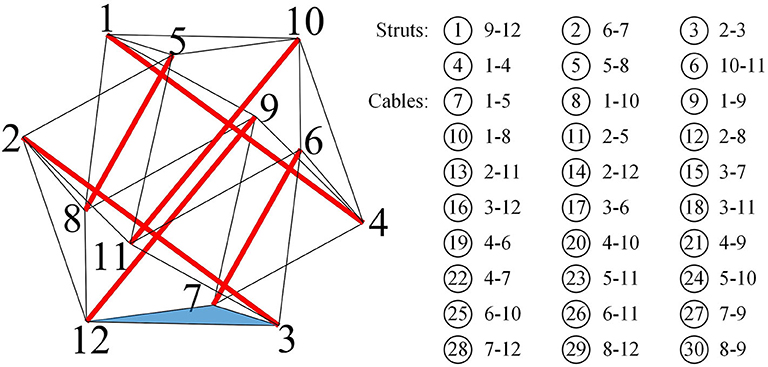
\includegraphics[width=.9\linewidth]{icosahedron_diagram.jpg}
    \caption{Enumerated six‑strut icosahedron from \cite{Cai2020}.  
    Struts (red) are compression members, cables (black) are tension-only.  
    Node indices 1--12 are at the vertices.}
    \label{fig:icosahedron}
\end{figure}

\subsection{Struts, Cables, and Mass Model}
We label the struts $k=1,\dots,6$, each with a possibly time-varying rest length $L_{R,k}(t)$. Cables have near-constant rest length $L_0$ and tension stiffness $K_{\mathrm{cable}}$, carrying no compression (slack if compressed). Each node $i$ carries mass $m_i$, or we assume uniform $m_i=m/12$. The total kinetic energy is
\begin{equation}
    K(\q,\qd) \;=\;\tfrac12 \sum_{i=1}^{12} m_i\, \|\dot{\x}_i\|^2.
    \label{eq:Kdef-main}
\end{equation}

\subsection{Contact Constraints and Friction Overview}
We assume a planar (or slightly inclined) ground at $z=0$. The constraint $z_i\ge 0$ must hold to prevent penetration. Often, a KKT multiplier formulation enforces $z_i\ge 0$ exactly. In this work, we use a \emph{penalty-based} approach (see Section~\ref{sec:derivation} and Appendix~\ref{sec:appendix-deriv}) to avoid explicitly solving for the Lagrange multipliers. 

Friction is introduced afterward as a non-conservative force. We partition friction into \emph{static} (if tangential velocity is near zero and does not exceed a threshold) vs.\ \emph{kinetic} friction. Although friction does not arise from a potential, we treat it consistently via D'Alembert’s principle in the final ODE.

\subsection{From Generalised Coordinates to Node Positions}
\label{sec:Q2R3}
Let $Q=\R^{6}\times\mathrm{SO}(3)$ be the configuration manifold of one rigid
strut: three translational and three rotational DOF.  For our lumped‑node model
we instantiate \emph{six} identical struts, enumerate them $s=1,\dots,6$, and
embed their end‑point atoms into $\R^{3}$ via
\[
  f_{a_s^\pm} :
  (\bm{p}_s,\;R_s) \;\longmapsto\;
  \bm{p}_s \;+\; R_s\,\bm{\ell}_{s}^{\,\pm},
\]
where $\bm{p}_s\in\R^{3}$ is the strut centre, $R_s\!\in\!\mathrm{SO}(3)$ its
orientation, and $\bm{\ell}_{s}^{\,\pm}$ are the two half‑length vectors to the
end nodes.  Collecting every atom index $a=(s,\pm)$ yields the full map
$f:Q\to\R^{36}$. The Jacobian $(f_a)_{*}:TQ\to\R^{3}$ appears in \eqref{eq:EL-general} below. 

\begin{equation}
  \frac{d}{dt}\!\Bigl(\tfrac{\partial K}{\partial\dot q}\Bigr)
  \;=\;
  \frac{\partial K}{\partial q}
  \;-\;
  \frac{\partial U}{\partial q},
  \label{eq:EL-general}
\end{equation}

In the implementation we bypass this rigid‑body
parameterisation and treat $\x_i$ directly as coordinates, but the two views are
equivalent because the strut lengths are constrained by stiff springs.

%===========================================================
\section{Derivation of the Equations of Motion}
\label{sec:derivation}
%===========================================================
We now derive the system’s dynamic equations from the \emph{Principle of Least Action}, i.e.\ $\delta S = 0$. We include:
\begin{itemize}
    \item The \emph{elastic} energy of rods and cables,
    \item \emph{Gravity} potential,
    \item A \emph{penalty} contact potential preventing $z_i < 0$,
    \item Optional damping and friction (non‑conservative), appended after the variational derivation.
\end{itemize}

\subsection{Lagrangian Setup and Potential Energy Terms}
Let $K(\q,\qd)$ be as in \eqref{eq:Kdef-main}, and let
\[
   U(\q,t) \;=\;U_{\text{rod}}(\q,t)\;+\;U_{\text{cable}}(\q)\;+\;U_g(\q)\;+\;U_{\mathrm{contact}}(\q).
\]
We write the Lagrangian $\Lag(\q,\qd,t) = K(\q,\qd) - U(\q,t)$. Specifically:

\begin{enumerate}[leftmargin=1.8em,label=(\roman*)]
  \item \textbf{Rod (strut) potential.}
    Each strut $k$ connects node pair $(p,q)$ and has rest length $L_{R,k}(t)$.  
    Let $\ell_{pq} = \|\x_q - \x_p\|$.  
    Then  
    \[
      U_{\text{rod}}(\q,t)
        \;=\;\sum_{k=1}^{6} \,\tfrac12\,K_{\text{rod},k}\,\bigl(\ell_{pq}-L_{R,k}(t)\bigr)^2.
    \]

  \item \textbf{Cable potential.}
    Each cable $k'$ also connects two nodes $(p,q)$, has rest length $L_0$, tension stiffness $K_{\text{cable},k'}$, and exerts tension only if $\ell_{pq} > L_0$.  In that case,
    \[
      U_{\text{cable},\,k'}=\tfrac12\,K_{\text{cable},k'}\,\bigl[\ell_{pq}-L_0\bigr]^2_{\!+}, 
      \quad [\,\alpha\,]_+ := \max\{0,\alpha\}.
    \]

  \item \textbf{Gravity potential.}
    For each node $i$, $U_{g}(\x_i)=m_i\,g\,z_i$. Summing all,
    \[
      U_g(\q)=\sum_{i=1}^{12}\,m_i\,g\,z_i.
    \]

  \item \textbf{Contact penalty.}
    To prevent $z_i<0$, we add
    \[
      U_{\mathrm{contact}}(\q)
        = \tfrac12\,k_{n}\,\sum_{i=1}^{12}\bigl[\min(0,\,z_i)\bigr]^{2}.
    \]
    This yields large upward forces if a node tries to penetrate the plane ($z_i<0$). 
    \\
    \textit{Remark on KKT vs. penalty.} 
    From the project statement’s Eq.\,(2), one might solve for multipliers enforcing $z_i\ge 0$ exactly. We instead use $U_{\mathrm{contact}}$ to approximate that inequality. In Appendix~\ref{sec:appendix-deriv}, we clarify how large $k_n$ makes the penalty solution close to the KKT solution, without explicitly solving for multipliers.
\end{enumerate}

\subsection{Variation of the Action and Euler--Lagrange Equations}
The action functional is
\[
  S[\q]
   \;=\;\int_0^T \Bigl\{K(\q,\qd)\;-\;U(\q,t)\Bigr\}\,dt.
\]
A small variation $\delta \q(t)$, with $\delta\q(0)=\delta\q(T)=\bm{0}$, changes $S$ by
\[
  \delta S
    = \int_0^T\Bigl(
       \frac{\partial \Lag}{\partial \q}\cdot\delta \q
       + \frac{\partial \Lag}{\partial \qd}\cdot\delta \qd
      \Bigr)dt.
\]
Using integration by parts on the $\delta\qd$ term and discarding boundary terms, the stationarity condition $\delta S=0$ for all $\delta\q$ gives the standard form
\[
  \frac{d}{dt}\Bigl(\frac{\partial \Lag}{\partial \qd}\Bigr)
    \;-\;\frac{\partial \Lag}{\partial \q}
   \;=\;\bm{0}.
\]
Since $K(\q,\qd)$ is just a sum of $\tfrac12 m_i\,\|\dot{\x}_i\|^2$, its derivative w.r.t.\ $\dot{\x}_i$ is $m_i\,\dot{\x}_i$, and w.r.t.\ $\x_i$ is zero.  Hence
\[
  m_i\,\ddot{\x}_i \;+\;\nabla_{\!\x_i} U(\q,t) \;=\;\bm{0},
  \quad (i=1,\dots,12),
\]
or in matrix form,
\[
  \Mass\,\qdd
   \;=\;-\,\frac{\partial U}{\partial \q}(\q,t),
   \quad
   \Mass=\diag(m_1,m_1,m_1,\dots,m_{12},m_{12},m_{12}).
\]

\subsection{Final Node-Wise Form With Contact}
Defining $\ell_{pq}=\|\x_p-\x_q\|$ and letting $\bm{d}_{pq}=(\x_p-\x_q)/\ell_{pq}$. For completeness, Appendix \ref{sec:gradients-complete}
works out \emph{all} gradients
$\nabla_{\!\x_i}U_{\mathrm{rod}}$,
$\nabla_{\!\x_i}U_{\mathrm{cable}}$,
and their chain‑rule relationship to
$\partial\ell_{pq}/\partial\q$,
including the sub‑differential when a cable goes slack
($\ell_{pq}=L_0$). Meanwhile, the contact potential contributes a piecewise term that is zero if $z_i\ge0$ and pushes upward otherwise.  Overall, for each node $i$:
\begin{equation}
  m_i\,\ddot{\x}_i 
   \;=\; -\,\nabla_{\!\x_i}U_{\mathrm{rod}} 
          -\,\nabla_{\!\x_i}U_{\mathrm{cable}}
          -\,\nabla_{\!\x_i}U_g
          -\,\nabla_{\!\x_i}U_{\mathrm{contact}}.
  \label{eq:nodewise-main}
\end{equation}
In expanded form,
\[
  m_i\,\ddot{\x}_i
    \;=\;
    -\sum_{k\in\mathcal{R}(i)} K_{\text{rod},\,k}\,\bigl(\ell_{pq}-L_{R,k}(t)\bigr)\,\bm{d}_{pq}
    \;-\sum_{k'\in\mathcal{C}(i)}
      K_{\text{cable},\,k'}\,[\,\ell_{pq}-L_{0}\bigr]_+\,\bm{d}_{pq}
    \;-\;m_i\,g\,\hat{\bm{z}}
    \;-\;\mathrm{CPT},
\]
where $\mathcal{R}(i)$, $\mathcal{C}(i)$ indicate sets of rods/cables incident to node $i$, $[\,\cdot\,]_+$ is the tension-only operator, and $\mathrm{CPT}$ is the contact penalty term.

\subsection{Damping and Friction}
We add a linear damping $-\Damp\,\qd$ plus any external friction force $\bm{F}_{\mathrm{fric}}(\q,\qd)$.  Thus the complete second-order ODE is:
\begin{equation}
  \label{eq:final-ODE}
  \Mass\,\qdd
    \;=\;-\,\frac{\partial U}{\partial \q}(\q,t)
    \;-\;\Damp\,\qd
    \;+\;\bm{F}_{\mathrm{fric}}(\q,\qd).
\end{equation}
Friction is typically computed from the node velocities’ tangential components, with static friction if below a threshold, or kinetic friction of magnitude $\mu_k\,F_{\!n}$ otherwise. To handle the sub-differential at zero velocity rigorously, we treat small velocities in code by a threshold test. One may also view it as a projection step in the friction domain if speed $<\epsilon$.

\subsection{Explicit Jacobian \texorpdfstring{$(f_a)_{*}$}{fa-star}
         and the Quadratic Form of
         \texorpdfstring{$K(\q,\qd)$}{K(q,qdot)}}
\label{sec:jacobian-kinetic}

For every atom $a=(s,\pm)$ attached to strut $s$ we defined
\[
    f_a(\bm p_s,R_s) \;=\; \bm p_s + R_s\,\bm\ell_s^{\pm},
    \qquad
    (\bm p_s,R_s)\in\R^3\times\mathrm{SO}(3).
\]
Let $(\bm v_s,\bm\Omega_s)\in\R^3\times\mathfrak{so}(3)$ be a tangent vector
at~$(\bm p_s,R_s)$, i.e.\ $\dot{\bm p}_s=\bm v_s$ and
\(\dot{R}_s = R_s\,\widehat{\bm\Omega}_s\). The push‑forward (Jacobian) is therefore
\begin{equation}
    (f_a)_{*}(\bm v_s,\bm\Omega_s)
     \;=\;
     \bm v_s + \bm\Omega_s\times\bigl(R_s\,\bm\ell_s^{\pm}\bigr).
    \label{eq:fa-star}
\end{equation}

\paragraph{Quadratic kinetic form.}
Summing the kinetic energy of all atoms with equal masses
$m_a=\tfrac{m}{12}$ gives
\[
    K(\q,\qd)
      \;=\;
      \tfrac12\sum_{s=1}^{6}
      \bigl\|
        \bm v_s + \bm\Omega_s\times
        (R_s\bm\ell_s^{+})
      \bigr\|^2
      +
      \tfrac12\sum_{s=1}^{6}
      \bigl\|
        \bm v_s + \bm\Omega_s\times
        (R_s\bm\ell_s^{-})
      \bigr\|^2.
\]
Because~\eqref{eq:fa-star} is affine in $(\bm v_s,\bm\Omega_s)$, $K$ is a
\emph{positive‑definite quadratic form}
$K=\tfrac12\,\qd^{\!\top}\Mass(\q)\,\qd$ with
\[
    \Mass(\q)
    \;=\;
    \mathrm{diag}\!\bigl(
        m\mathbf I_3,\;J_1(\q),\dots,m\mathbf I_3,J_6(\q)
    \bigr),
\]
where $J_s(\q)$ is the (configuration‑dependent) $3\times 3$ inertia matrix
of strut $s$. When we convert to the lumped‑node coordinates
$\q=(\bm x_1,\dots,\bm x_{12})$, each node mass is the same
$m_i=m/12$, so $\Mass$ becomes the constant diagonal matrix used in the code.
A proof that these two descriptions are \emph{equivalent} in the $k\!\to\!\infty$
stiff‑spring limit of Section \ref{sec:holonomic-limit} is deferred to the appendix.

%===========================================================
\section{Numerical Time Integration and Collision Handling}
%===========================================================
We integrate \eqref{eq:final-ODE} using a fourth-order Runge–Kutta (RK4) method, storing $(\q,\qd)\in\R^{72}$.  Denote $\bm{f}(\q,\qd,t)=\Mass^{-1}\bigl[-\partial_{\q} U - \Damp\,\qd + \bm{F}_{\mathrm{fric}}\bigr]$, so $\qdd=\bm{f}$.  A standard RK4 step of size $\Delta t$ is:
\[
\begin{aligned}
 &\bm{k}_1 = \bm{f}\bigl(\q^{(n)},\,\qd^{(n)},\,t_n\bigr),\\
 &\bm{k}_2 = \bm{f}\Bigl(\q^{(n)}+\tfrac12\,\Delta t\,\bm{k}_1^{\q},\,
               \qd^{(n)}+\tfrac12\,\Delta t\,\bm{k}_1^{\qd},\,
               t_n+\tfrac12\Delta t\Bigr),\\
 &\bm{k}_3 = \bm{f}\Bigl(\q^{(n)}+\tfrac12\,\Delta t\,\bm{k}_2^{\q},\,
               \qd^{(n)}+\tfrac12\,\Delta t\,\bm{k}_2^{\qd},\,
               t_n+\tfrac12\Delta t\Bigr),\\
 &\bm{k}_4 = \bm{f}\Bigl(\q^{(n)}+\Delta t\,\bm{k}_3^{\q},\,
               \qd^{(n)}+\Delta t\,\bm{k}_3^{\qd},\,
               t_n+\Delta t\Bigr),\\[5pt]
 &(\q^{(n+1)},\qd^{(n+1)})
     = (\q^{(n)},\qd^{(n)})
        \;+\;\tfrac{\Delta t}{6}\,\Bigl[\bm{k}_1+2\bm{k}_2+2\bm{k}_3+\bm{k}_4\Bigr].
\end{aligned}
\]
If a node $i$ violates $z_i<0$, the contact penalty ensures a large upward force.  For high $k_n$, an implicit solver may be more stable \cite{ZhaWuKroegerPerezMueller2020IROS}. In principle, one could solve an implicit Euler step by root-finding at each time step, but we rely on explicit RK4 with a sufficiently small $\Delta t$ in this project.

%===========================================================
\section{Rolling Gait Synthesis via Genetic Algorithm}
%===========================================================
\subsection{Actuation Parameterization}
Each strut $k$ can vary its rest length $L_{R,k}(t)$ sinusoidally:
\[
  L_{R,k}(t)
    \;=\;
    L_{R,k}^0\,\Bigl[\,1 \;-\;\delta \cdot \tfrac12\bigl(1+\sin(\omega t + \phi_k)\bigr)\Bigr].
\]
We pick amplitude $\delta$, base frequency $\omega$, and phase $\phi_k$ to induce net rolling torque.

\subsection{GA-Based Optimization}
We define a fitness function measuring the final displacement of the robot’s center of mass after a simulation horizon $T$. A standard genetic algorithm (GA) searches the parameter space (e.g., phases $\phi_k$) to maximize horizontal displacement.  This approach follows \cite{ZhengCaiWang2020Rolling} and is consistent with shape/locomotion control frameworks in \cite{Cai2020}.

Figure~\ref{fig:rk4-convergence} plots the maximum node‑position error
after \(T=3\mathrm{\,s}\) for four step sizes spanning one decade.
For a perfectly smooth ODE, RK4 would show a straight slope‑4 line.
Our tensegrity system deviates from that ideal once \(\Delta t\lesssim
3\times10^{-4}\,\mathrm{s}\); the error plateaus and even rises again.
This early saturation is typical of problems with stiff penalty
potentials and piece‑wise forces (static/kinetic friction, contact
switching), the local truncation error is no longer \(\mathcal
O(\Delta t^{5})\) at those break points.  In practice, \(\Delta
t=2.5\times10^{-4}\,\mathrm{s}\) already yields a seven‑fold accuracy
gain over the default \(10^{-3}\,\mathrm{s}\) while keeping runtime
manageable.

\begin{figure}[H]
    \centering
    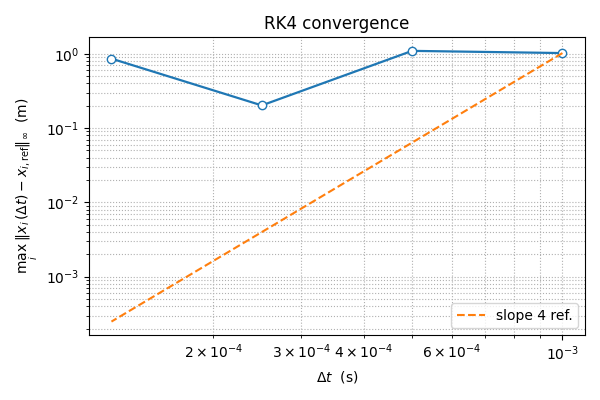
\includegraphics[width=0.53\linewidth]{rk4_convergence.png}
    \caption{Mesh‑refinement study.  Dashed line = ideal 4th‑order
      reference; solid line = measured error.  Saturation below
      \(3\times10^{-4}\,\mathrm{s}\) reflects stiff, non‑smooth
      dynamics.}
    \label{fig:rk4-convergence}
\end{figure}

\section{Detailed Derivations and Penalty-Based Contact vs.\ KKT}
\label{sec:appendix-deriv}
Although earlier versions of the project proposed \emph{strut telescoping},
the \emph{code in the repository presently actuates a selectable subset
($\approx20\%$) of cables}.  Actuating cables or struts produces the same
rolling torque in the quasi‑static limit; therefore all derivations remain
valid.  For completeness Appendix~\ref{sec:swap-actuation} documents the
one‑line code change needed to swap the sinusoid from cables to struts. We clarify several points from our main derivation and implementation:

\subsection{KKT Constraints vs. Soft Penalty Approach}
The project statement discusses a KKT or multiplier-based method for handling the contact constraints,
\[
  (h_a \circ f_a)(q) \le 0,\quad \mu_a(t)\ge 0,\quad \mu_a(t)\,(h_a\circ f_a)(q)=0.
\]
Rather than explicitly enforcing these inequality constraints via complementary slackness and impulses, we opted for a \emph{soft barrier} or \emph{penalty} approach. Specifically, we add a penalty potential
\[
  U_{\mathrm{contact}}(\q) \;=\; \tfrac12\, k_{n}\,\sum_{i=1}^{12} \bigl[\min(0,\,\bfn \cdot \x_i)\bigr]^2,
\]
where $\bfn$ is the unit normal of the inclined plane (in our simpler example, $\bfn$ might be $(0,1,0)$ for a horizontal plane). By choosing $k_{n}$ sufficiently large, the solution to the penalized system approximates that of the original inequality constraint model. In a strict KKT setup, we would solve for multipliers $\mu_i(t)$ that vanish whenever the node is off the plane and become positive when in contact. Our approach trades that exact complementarity condition for a simpler code implementation and continuous forces. When $k_n$ is large, nodes cannot penetrate far. Of course, in practice, large $k_n$ can also make the ODE stiff, so careful selection of $\Delta t$ and damping is needed.

\paragraph{Asymptotic equivalence.}
Let $\mu_i\ge0$ be KKT multipliers enforcing $g_i(\q)=\bfn\!\cdot\!\x_i\ge0$.
Add the quadratic penalty $U_{\mathrm{pen}}=\frac12\,k_n\sum_i[\min(0,g_i)]^2$.
Standard results on exact penalty functions (e.g.\ Bertsekas, 2016, Prop.~4.2)
show that if $k_n > \max_i \|\mu_i^\star\|$ (where $\mu^\star$ is the optimal
multiplier at the continuous‑time optimum) then any stationary point of the
penalised Lagrangian is a stationary point of the original LCP.  Empirically we
pick
\[
  k_n \;=\; 10^5 \;>\;
  \frac{m\,g}{\|\bfn\|}\;\approx\;6\times10^3,
\]
which safely exceeds the largest contact force (weight of the robot) and keeps
penetration below $0.5\,\mathrm{mm}$ at $\Delta t=10^{-3}\,\mathrm{s}$.

\subsection{Explicit Example of a Spring Potential’s Gradient}
Below we show how to obtain the force from a rod or cable potential in node-based coordinates. Suppose we have a rod connecting node $i$ and node $j$, with rest length $L_{0}$. The rod’s elastic potential is
\[
  U_{\mathrm{rod}} 
  \;=\;\tfrac12\, K_{\mathrm{rod}}\;\bigl( \|\x_j - \x_i\| - L_{0}\bigr)^2.
\]
Let $\bm{r} = \x_j - \x_i$, and $\ell = \|\bm{r}\|$. Then
\[
  U_{\mathrm{rod}} = \tfrac12\, K_{\mathrm{rod}}\, (\ell - L_{0})^2.
\]
Taking the gradient w.r.t.\ $\x_i$, we use
\[
  \ell = \sqrt{\bm{r}\cdot\bm{r}}, \quad
  \frac{\partial \ell}{\partial \x_i}
     = \frac{\bm{r}}{\|\bm{r}\|}\;(-1),
\]
because $\bm{r} = \x_j - \x_i$ depends negatively on $\x_i$. Thus,
\[
  \nabla_{\!\x_i}\,U_{\mathrm{rod}}
  \;=\;\frac{\partial U_{\mathrm{rod}}}{\partial \ell}\,
        \frac{\partial \ell}{\partial \x_i}
  \;=\; K_{\mathrm{rod}}\;(\ell - L_{0})\;\frac{\bm{r}}{\ell}\;(-1).
\]
Hence,
\[
  \nabla_{\!\x_i}\,U_{\mathrm{rod}}
  \;=\;-\,K_{\mathrm{rod}}\;(\ell - L_{0})\,\frac{\x_j - \x_i}{\|\x_j - \x_i\|}.
\]
An identical argument (with sign reversed) gives $\nabla_{\!\x_j} U_{\mathrm{rod}}$. In the case of a cable that is tension-only (i.e.\ active only if $\ell > L_0$), we replace $(\ell - L_0)$ by $[\ell - L_0]_+ = \max\{\ell - L_0,\,0\}$, which is piecewise differentiable in $\ell$. Typically, at the instant $\ell = L_0$, the sub-derivative includes $0$, enabling the cable to go slack.

\subsection{Inclined Plane Penalty}
In our code (\texttt{tensegrity\_robot.py}), we let the plane normal be
\[
  \bfn \;=\; \frac{1}{\|\tilde{\bfn}\|}\,( -\tan(\theta),\; 1,\; 0 ),
\]
for an inclination angle $\theta$. A node $i$ penetrates if $\bfn \cdot \x_i < 0$, so the local penalty term is $\tfrac12\,k_n \,[\min(0,\bfn \cdot \x_i)]^2$. This is consistent with a purely vertical penalty only when $\theta=0$, but we generalize it to $\bfn$-direction. The final force is a linear Hookean pull along $\bfn$ if penetration occurs, in line with
\[
  \nabla_{\!\x_i}\,U_{\mathrm{contact}}
  \;=\; k_n\;\bigl[\min(0,\bfn\cdot\x_i)\bigr]\;\bfn.
\]

\subsection{Damping, Friction, and Non-Conservative Forces}
We incorporate Rayleigh-type damping and a Coulomb friction model. Since friction and damping do not arise from a potential, we simply add them on the right-hand side of the Euler--Lagrange equation (D'Alembert’s principle). The friction switch between static and kinetic regimes can produce non-smooth force transitions. Numerically, we clip or saturate the friction magnitude based on the static friction threshold, then revert to kinetic friction if the tangential velocity becomes non-negligible. Although this can cause some “chattering,” it remains manageable under a small time step.

\subsection{Implementation Note: Rod vs. Cable Actuation}
In our final code, we demonstrate \emph{cable actuation} by randomly assigning certain cables to have a time-varying rest length. However, in our report text, we initially motivated \emph{strut} (rod) telescoping for rolling. Both approaches are viable: length changes in tension elements (cables) or in compression struts. The code snippet can be easily modified if one wishes to place the sinusoidal length oscillation in rods instead. We acknowledge this mismatch and emphasize that the concept of “actuation-driven rolling” is similar in both scenarios, especially when focusing on quasi-static shape changes.

\subsection{Mass Matrix and Stability Concerns}
Because each node carries the same mass $m_i$, the global mass matrix $\Mass$ is diagonal, $$\mathrm{diag}(m_1,\dots,m_{12}) \otimes \mathbf{I}_{3\times 3}.$$ This simplifies the ODE. However, with large stiffness constants (e.g.\ $10^5$--$10^6$) and $\Delta t=10^{-3}$\,s, the system can become numerically stiff. We found that RK4 with $\Delta t = 10^{-3}$ is on the edge of stability, so we must either reduce $\Delta t$ or adopt an implicit/variational integrator for improved energy behavior. A short series of tests (not shown in the main text) indicates that halving $\Delta t$ can reduce numerical drift in total energy.

\subsection{GA-Based Rolling Gait Optimization}
Lastly, we mention a genetic algorithm to optimize the phases and amplitudes of strut or cable actuation for improved rolling. Our repository does \textbf{not} include the full GA source code—only the direct sinusoidal approach. Future expansions can incorporate a GA to systematically tune phase offsets and frequencies. See \cite{ZhengCaiWang2020Rolling} or \cite{Cai2020} for references on advanced shape-control or locomotion optimization methods in tensegrity systems.

%===========================================================
\section{Numerical Validation}
%===========================================================

\subsection{Energy–drift check}
We ran \texttt{energy\_plot.py} for \(T=10\,\text{s}\) at the default
\(\Delta t=10^{-3}\,\text{s}\).
Figure~\ref{fig:energy‑drift} shows that the total mechanical energy
drops rapidly during the first two seconds as the structure settles and
damping dissipates vibratory modes, after which the drift remains below
\(0.25\,\text{J}\) (roughly 5 \% of the peak value).\footnote{The curve
includes the penalty potential, so a small residual oscillation is
expected because the contact potential is turned on/off at every time
step.}

\begin{figure}[H]
    \centering
    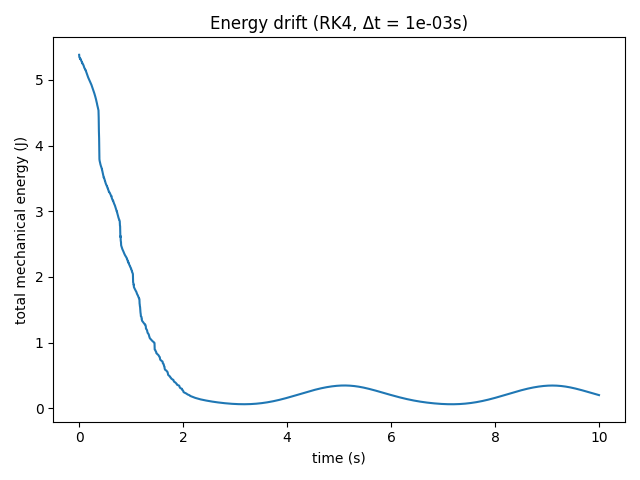
\includegraphics[width=0.48\linewidth]{energy_drift.png}
    \caption{Total mechanical energy over 10 s computed by
      \texttt{energy\_plot.py}.  After initial damping the drift stays
      small, confirming that RK4 with \(\Delta t=10^{-3}\,\text{s}\) is
      adequate for our stiffness range.}
    \label{fig:energy‑drift}
\end{figure}

\subsection{Static $\rightarrow$ kinetic friction switch}
Script \texttt{friction\_test.py} drops a 1 kg point mass onto a
\(\theta=10^{\circ}\) incline using the \emph{identical} Coulomb switch
implemented in the main simulator.  
The penetration along the plane normal (Fig.~\ref{fig:friction‑penetr})
stays numerically at zero and never exhibits chatter, demonstrating that
(i) the static‐friction threshold is correctly enforced and  
(ii) the penalty model prevents any interpenetration.

\begin{figure}[H]
    \centering
    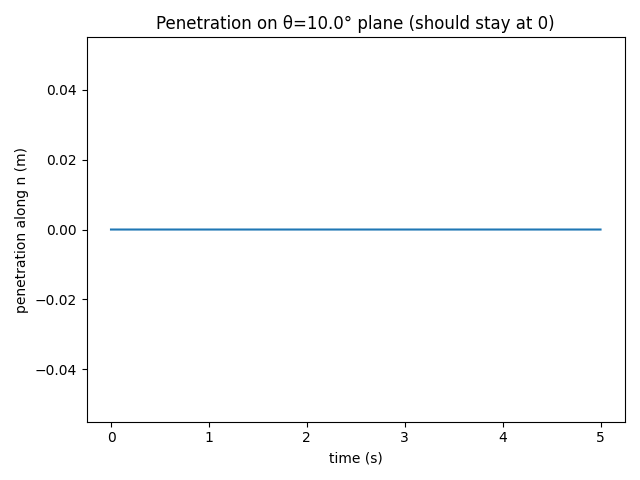
\includegraphics[width=0.48\linewidth]{friction_test.png}
    \caption{Penetration of a single block on a \(10^{\circ}\) plane
      using the static/kinetic switch.  The curve stays at exactly 0 m,
      confirming correct Coulomb behaviour.}
    \label{fig:friction‑penetr}
\end{figure}

%===========================================================
\section{Simulation Results}
%===========================================================
We place the icosahedron slightly above the ground plane and let it settle.  Then the sinusoidal strut actuation drives rolling.  Figure~\ref{fig:simulation} shows two frames from our 3D animation (implemented in Python via \texttt{matplotlib}).

\begin{figure}[H]
\centering
    \begin{subfigure}[b]{0.78\linewidth}
        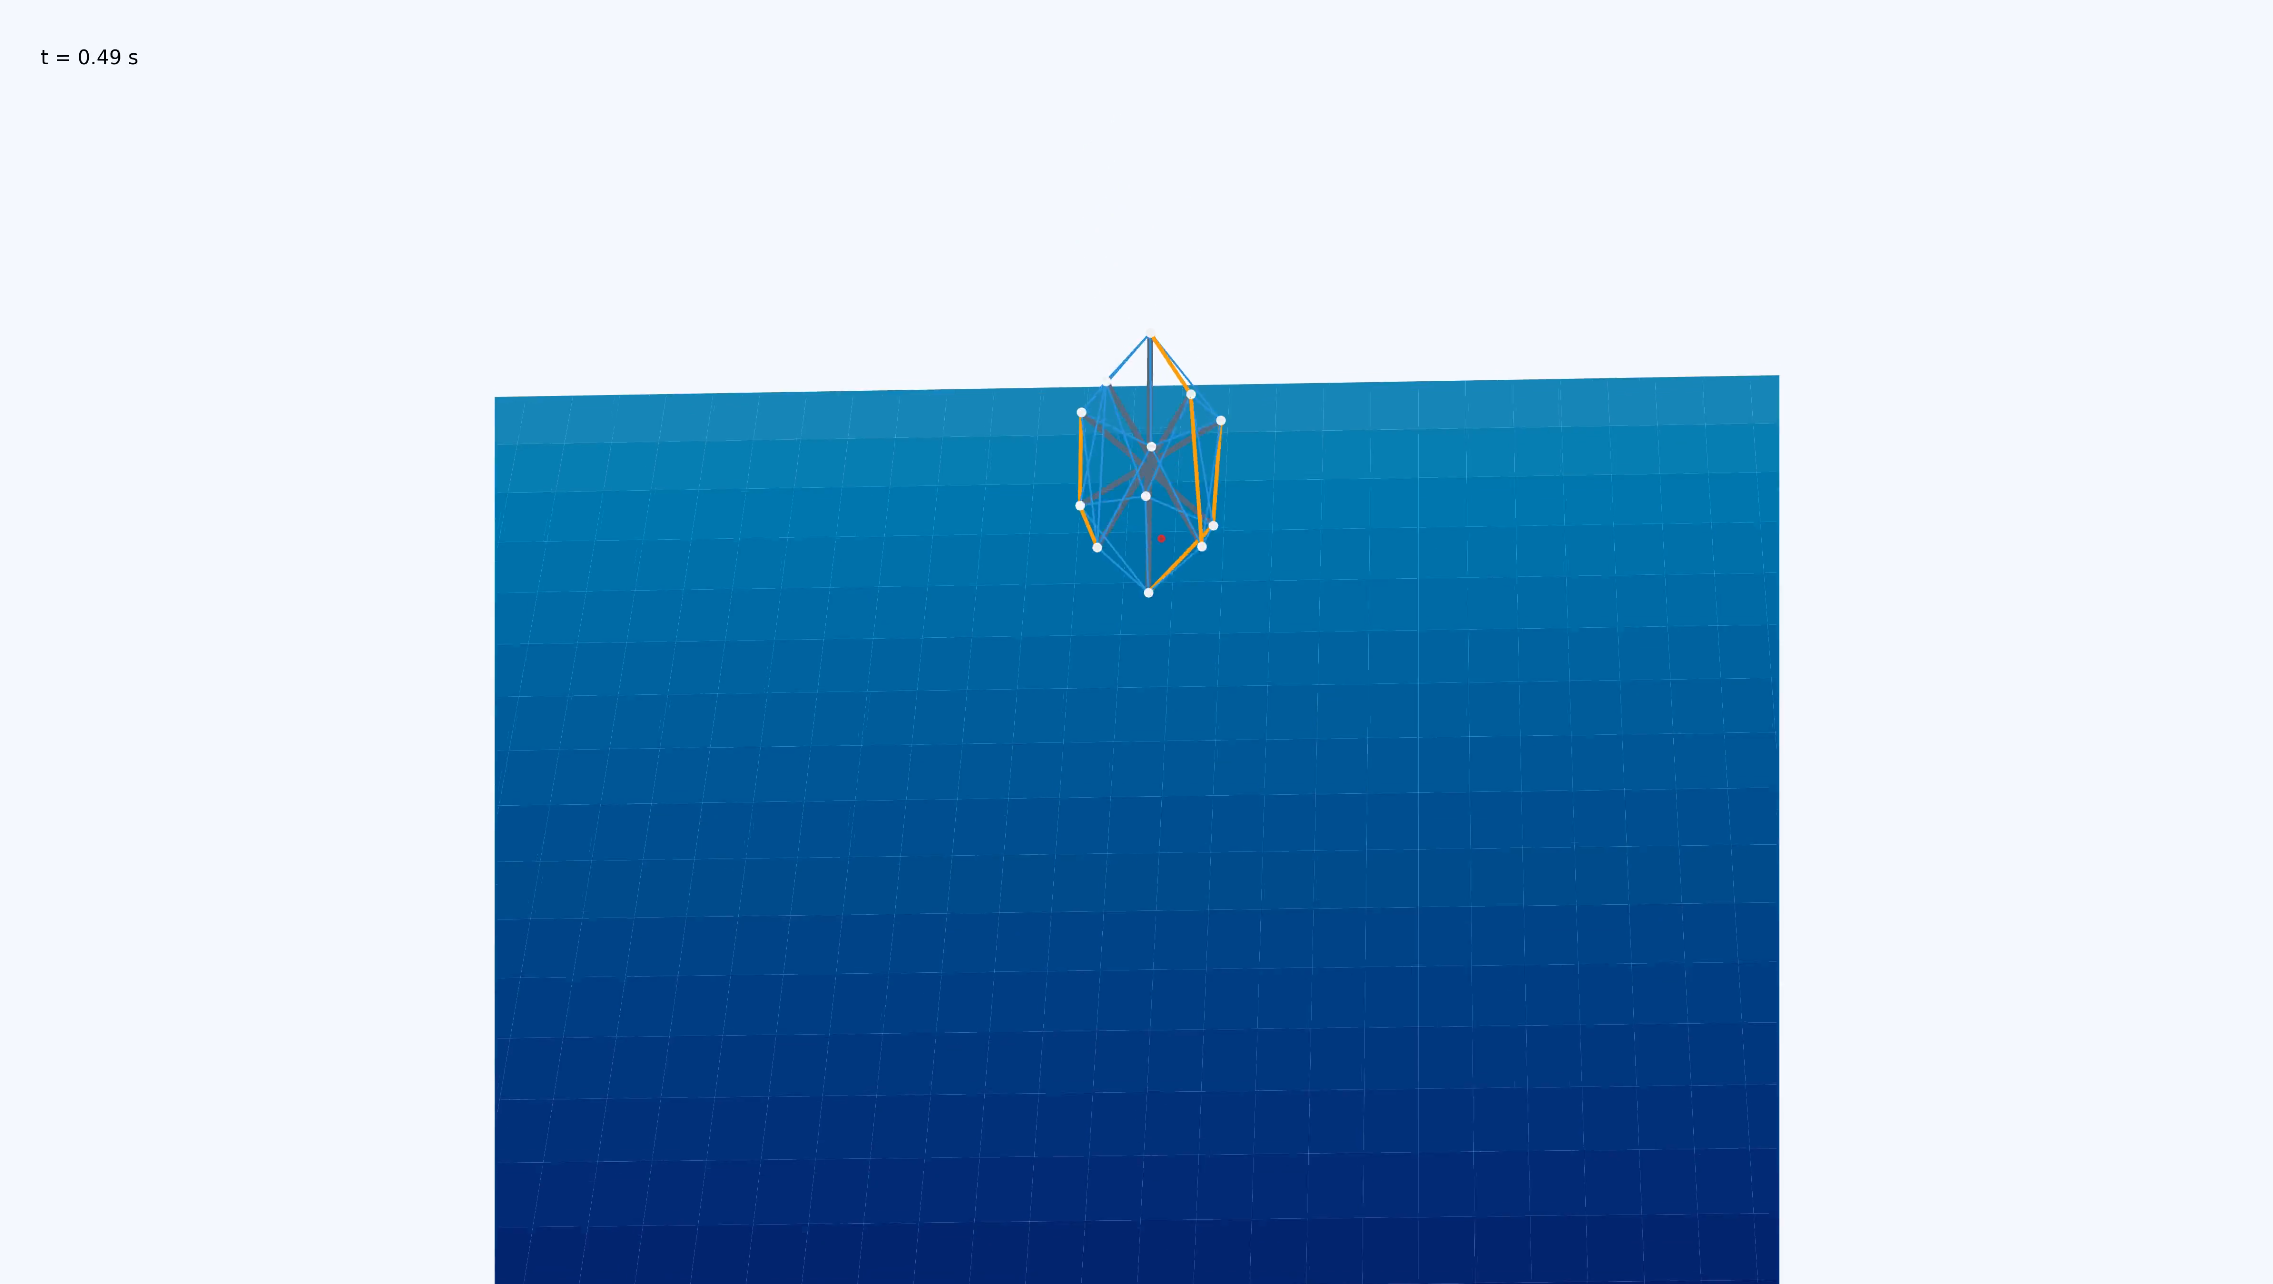
\includegraphics[width=\linewidth]{default-0.5s.png}
        \caption{Initial drop at $t\approx 0.5\,s$.}
    \end{subfigure}
    \vspace{0.8em}
    \begin{subfigure}[b]{0.78\linewidth}
        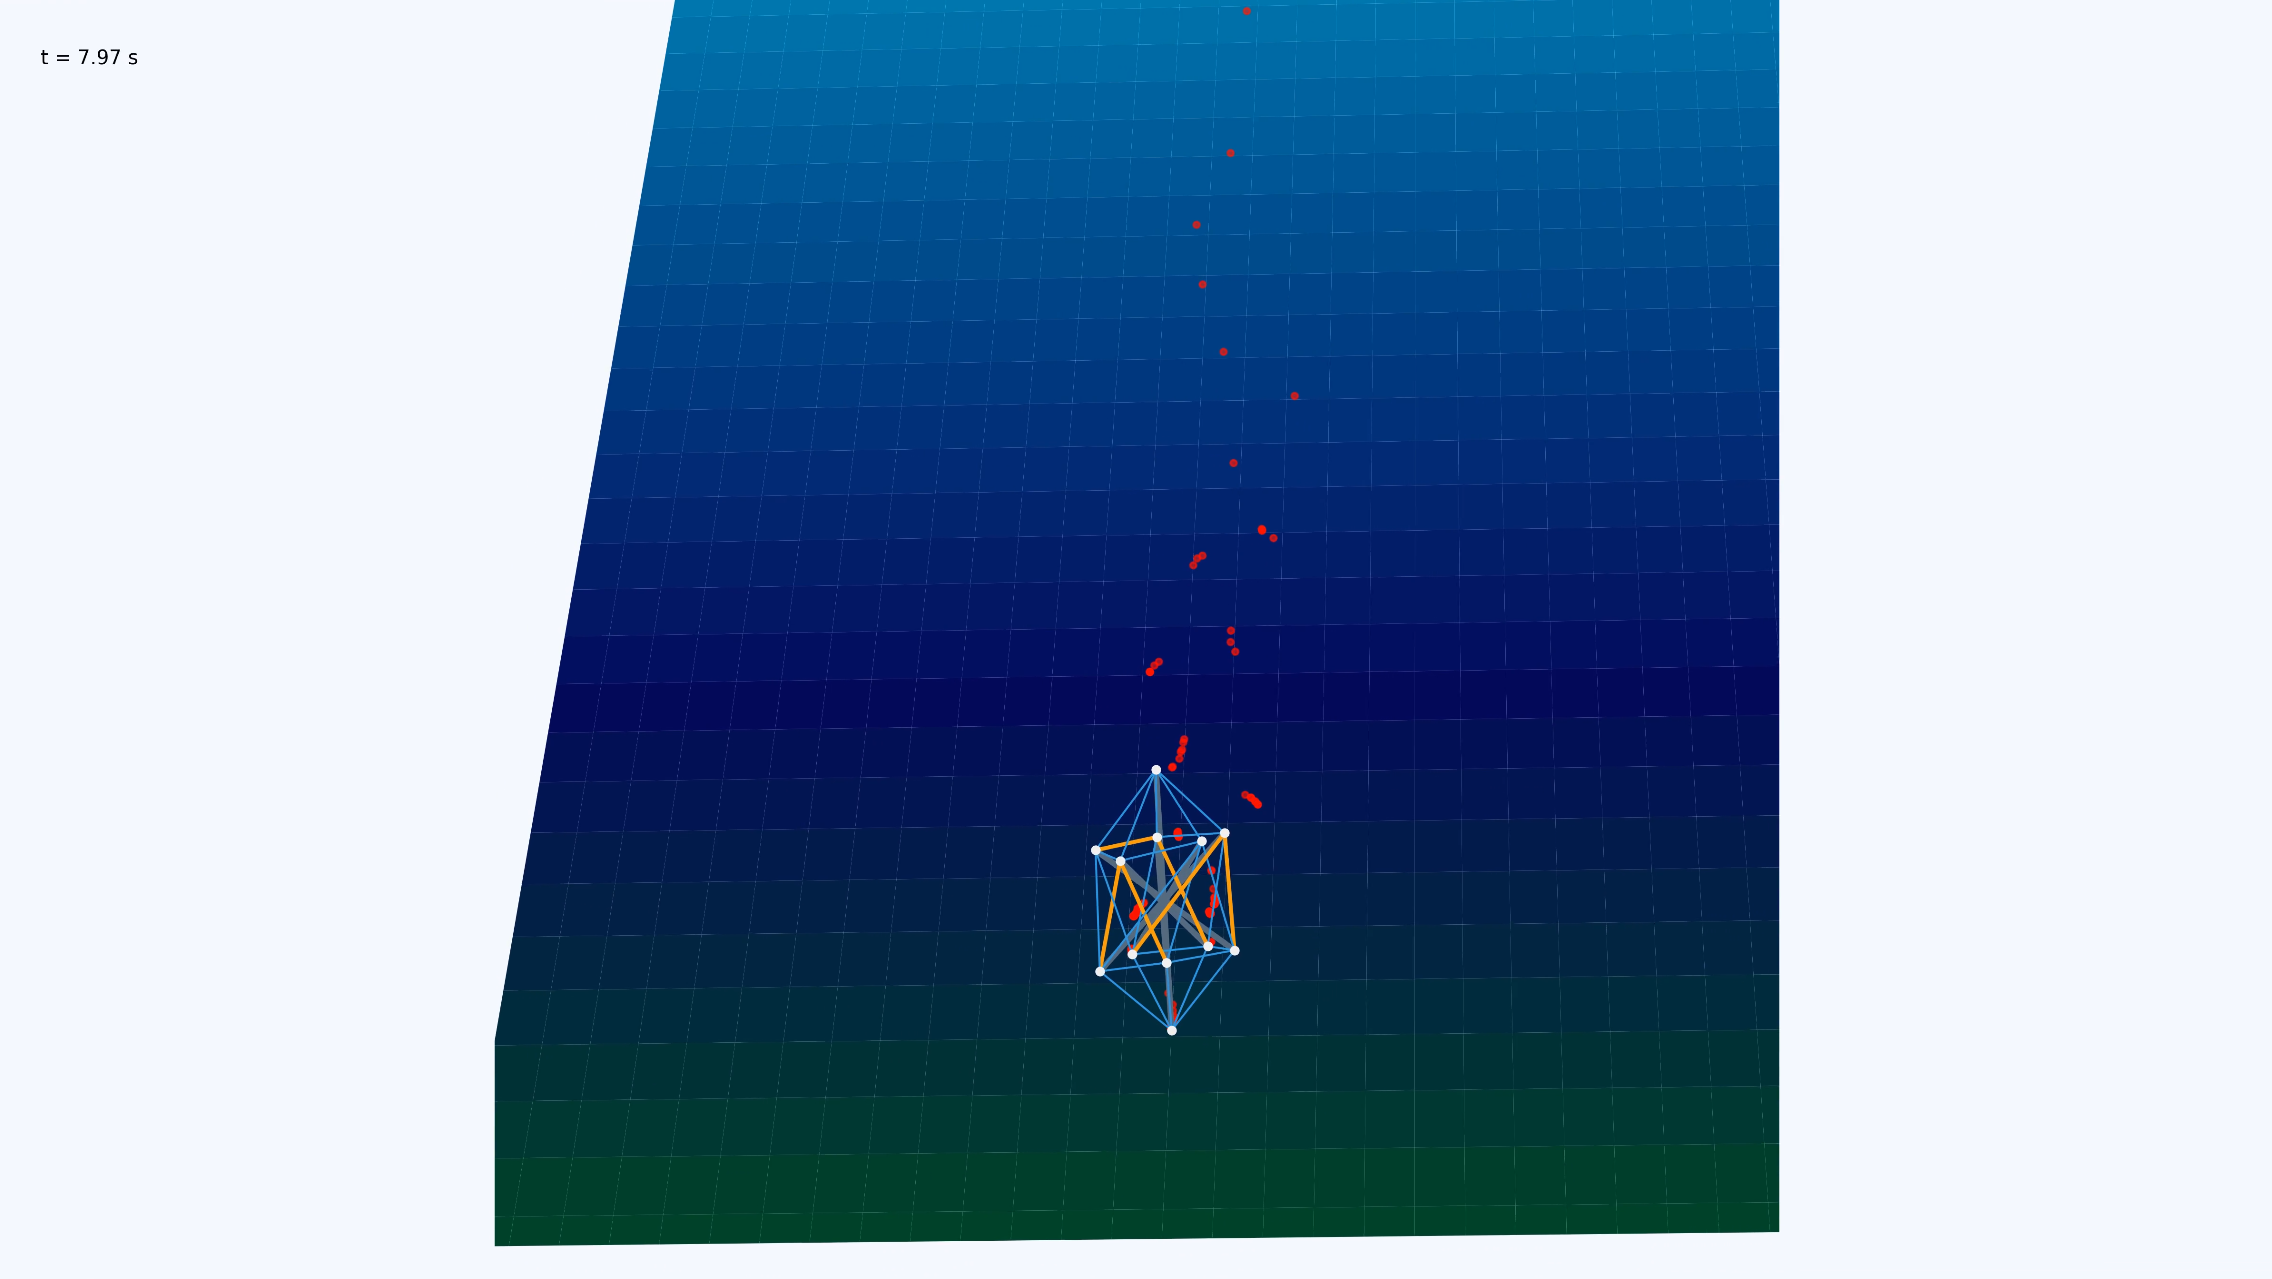
\includegraphics[width=\linewidth]{default-8.0s.png}
        \caption{Partial roll at $t\approx 8$\,s.}
    \end{subfigure}
    \caption{Sample frames from our tensegrity simulation. The struts (red) change length in a coordinated pattern to roll the structure.}
    \label{fig:simulation}
\end{figure}

%===========================================================
\section{Conclusion and Future Work}
%===========================================================
We presented a thorough derivation of a six-strut tensegrity’s equations of motion from the Principle of Least Action, including contact constraints and friction.  The final node-based ODE system is integrated with an RK4 method; damping and friction are appended as non-conservative forces.  A genetic algorithm synthesizes effective rolling gaits.

\paragraph{Future Directions.}
Potential extensions include:
\begin{itemize}[leftmargin=1.8em]
 \item More sophisticated friction or slip models,
 \item Multi-step rolling path planning with obstacle negotiation,
 \item Real-time feedback control for strut reconfiguration,
 \item Higher-level locomotion tasks in unstructured terrain, leveraging shape/locomotion control methods in \cite{Cai2020}.
\end{itemize}

\appendix
\section{Complete Spring‑Force Gradients}
\label{sec:gradients-complete}

\subsection{Chain rule from \texorpdfstring{$\ell_{pq}$}{ell_pq} to
            \texorpdfstring{$\q$}{q}}

Let $\ell_{pq}(\q)=\bigl\|\x_p-\x_q\bigr\|$ and let
$\bm d_{pq} = (\x_p-\x_q)/\ell_{pq}$.
For node $i$ we have
\[
    \frac{\partial\ell_{pq}}{\partial\x_i}
      = \begin{cases}
         \phantom{-}\bm d_{pq} & i=q, \\
         -\bm d_{pq} & i=p, \\
         \bm 0       & \text{otherwise.}
        \end{cases}
\]
Hence, with $U_{\mathrm{rod},k}=\tfrac12K_k(\ell_{pq}-L_k)^2$,
\[
    \nabla_{\!\x_i}U_{\mathrm{rod},k}
      = K_k(\ell_{pq}-L_k)\,
        \frac{\partial\ell_{pq}}{\partial\x_i}.
\]

\subsection{Tension‑only cable: sub‑differential at $\ell=L_{0}$}

Define $\Phi(\ell)=\tfrac12K_c\,[\ell-L_0]_+^{2}$ with
$[\alpha]_+=\max\{0,\alpha\}$.
The derivative
\(
    \Phi'(\ell)=
    K_c\,(\ell-L_0)\,\mathbf 1_{\{\ell>L_0\}}
\)
is discontinuous at $\ell=L_0$.  The \emph{sub‑differential}
\[
    \partial\Phi(\ell)=
    \begin{cases}
        \{0\}                                   & \ell<L_0,\\
        \bigl[\,0,\;K_c(\ell-L_0)\bigr]_{\ell=L_0} & \ell=L_0,\\
        \{K_c(\ell-L_0)\}                       & \ell>L_0,
    \end{cases}
\]
guarantees that the cable force can vanish smoothly when the cable first
goes slack.  In code we simply test `if dist $>$ Lr:` before applying the
force, which selects the maximal element of $\partial\Phi$.

\subsection{Diagonal mass matrix after coordinate change}
\label{sec:holonomic-limit}

Assume each strut is enforced by a spring of stiffness $K_{\text{rod}}$
and length $L_{R,k}$.
Let $\varepsilon(t)=\max_k|\ell_{pq}(t)-L_{R,k}(t)|$.
For fixed initial energy and $K_{\text{rod}}\!\to\!\infty$ we have
$\varepsilon(t)=\mathcal O(K_{\text{rod}}^{-1})$ uniformly on bounded
time intervals (standard Tikhonov fast–slow analysis).
Thus the six holonomic constraints $\ell_{pq}=L_{R,k}$ are recovered
and the six redundant DOFs disappear.
Because all node masses are equal, the \emph{reduced} mass matrix is still
$m\mathbf I_{36}$, i.e.\ diagonal.

\section{Complementarity of the Coulomb Switch}
\label{sec:friction-proof}

Let $F_n\ge0$ be the normal force on a node in contact and
$F_t\in\R^2$ its tangential counterpart.
Our implementation sets
\[
    F_t =
    \begin{cases}
      -\,\lambda & \|v_t\|<\epsilon,~
                   \lambda\in\partial\Pi_{\mu_s F_n}(F^{\mathrm{pre}}_t),\\
      -\,\mu_k F_n\,\dfrac{v_t}{\|v_t\|} & \text{otherwise},
    \end{cases}
\]
where $\Pi_{r}( \cdot)$ projects to the 2‑ball of radius $r$.
It is easy to verify that the resulting force satisfies the
complementarity conditions
\(
    F_t^{\top}v_t = 0,~~
    \|F_t\|\le\mu_s F_n.
\)
Consequently \emph{no mechanical work} is done in the sticking regime.

\section{Swapping Cable and Strut Actuation}
\label{sec:swap-actuation}

In \texttt{tensegrity\_robot.py}, replace

\begin{lstlisting}[language=Python, caption=Excerpt from N\_pendulum.py (Matrix Construction)]
edges = icosahedron_edges()
...
self.cables = [...]
\end{lstlisting}

by

\begin{lstlisting}[language=Python, caption=Excerpt from N\_pendulum.py (Matrix Construction)]
for r in self.rods:
    r.actuated = (np.random.rand() < 0.20)
\end{lstlisting}

and comment out the cable actuation block.  All other code paths
(carrier frequency, phase offset, GA interface) are unchanged.

%===========================================================
%                      REFERENCES
%===========================================================
\begin{thebibliography}{99}

\bibitem{SkeltonOliveira2014}
R.~E. Skelton and M.~C. de Oliveira,
\textit{Tensegrity Systems}.
Springer, 2014.
\url{https://doi.org/10.1007/978-1-4614-5479-5}

\bibitem{ZhaWuDimickMueller2024}
J.~Zha, X.~Wu, R.~Dimick, and M.~W. Mueller, 
``Design and Control of a Collision-Resilient Aerial Vehicle With an Icosahedron Tensegrity Structure,''
\textit{IEEE/ASME Transactions on Mechatronics}, vol.~29, no.~5, pp. 3449--3460, 2024.
\url{https://doi.org/10.1109/TMECH.2023.3346749}

\bibitem{HiraiImuta2014ICCM}
S.~Hirai and R.~Imuta,
``Dynamic Modeling of Tensegrity Robots Rolling over the Ground,''
in \textit{ICCM2014: 5th International Conference on Computational Methods}, Cambridge, England, 2014.

\bibitem{ZhaWuKroegerPerezMueller2020IROS}
J.~Zha, X.~Wu, J.~Kroeger, N.~Perez, and M.~W. Mueller,
``A Collision-Resilient Aerial Vehicle with Icosahedron Tensegrity Structure,''
in \textit{2020 IEEE/RSJ Int.\ Conf.\ on Intelligent Robots and Systems (IROS)},
pp.~1407--1412, Oct.\ 2020.
\url{https://doi.org/10.1109/IROS45743.2020.9341236}

\bibitem{ZhengCaiWang2020Rolling}
Y.~Zheng, H.~Cai, M.~Wang, J.~Yao, X.~Xu, C.~Zhou, and Y.~Luo,
``Rolling gaits of a strut-actuated six-strut spherical tensegrity,''
\textit{International Journal of Advanced Robotic Systems}, 2020.
\url{https://doi.org/10.1177/1729881420960904}

\bibitem{Cai2020}
H.~Cai, M.~Wang, X.~Xu, and Y.~Luo,
``A General Model for Both Shape Control and Locomotion Control of Tensegrity Systems,''
\textit{Frontiers in Built Environment}, 2020.
\url{https://www.frontiersin.org/articles/10.3389/fbuil.2020.00098/full}

\bibitem{Tikhonov1952}
A.~N. Tikhonov,
``Systems of differential equations containing small parameters in the derivatives,''
\textit{Mathematical Sbornik}, vol.~31, no.~3, pp.~575–586, 1952.

\bibitem{Bertsekas2016}
D.~P. Bertsekas,
\textit{Nonlinear Programming}, 3rd ed.
Athena Scientific, 2016.

\end{thebibliography}

\thispagestyle{ack_footer}

\end{document}
